\documentclass[a4paper,oneside]{article}

\usepackage[utf8]{inputenc}
\usepackage[brazil]{babel}
\usepackage{bookman}
\usepackage{ulem}
\usepackage{amssymb}
\usepackage{amsthm}
\usepackage{amsmath}
\usepackage{mathrsfs}
\usepackage{xspace}
\usepackage{enumerate}
\usepackage{makeidx}
\usepackage{calc}
\usepackage{ifthen}
\usepackage{epsfig}
\usepackage[portugues,vlined,boxruled,linesnumbered]{algorithm2e}

\setlength{\headheight}{0mm}
\setlength{\headsep}{0mm}
\setlength{\textheight}%
  {\paperheight-\footskip-\headsep-\headheight-\topmargin-\voffset-2in}
\setlength{\marginparwidth}{0mm}
\setlength{\marginparsep}{0mm}
\setlength{\textwidth}%
  {\paperwidth-\marginparwidth-\marginparsep-\oddsidemargin-\hoffset-2in}

\def\MMe{\mathrm{e}}
\def\MMi{\mathrm{i}}
\def\MMd{\mathrm{d}}
\def\MMN{\mathbb{N}}
\def\MMZ{\mathbb{Z}}
\def\MMQ{\mathbb{Q}}
\def\MMQbar{\overline{\mathbb{Q}}}
\def\MMR{\mathbb{R}}
\def\MMC{\mathbb{C}}
\def\MMP{\mathbb{P}}
\def\MME{\mathbb{E}}
\def\MMp{\mathrm{.}}
\def\MMv{\mathrm{,}}
\def\MMpv{\mathrm{;}}
\def\Hdie{\mathscr{H}}
\def\Rdie{\mathscr{R}}
\def\Var{\mathrm{Var}}
\def\geq{\geqslant}
\def\leq{\leqslant}
\def\divd{\backslash}
\def\ndivd{\not{\backslash}}
\def\parenteses#1{\left(#1\right)}
\def\colchetes#1{\left[\,#1\,\right]}
\def\colc#1{\colchetes{#1}}
\def\chaves#1{\left\{#1\right\}}
\def\cardi#1{\left|\,#1\,\right|}
\def\chao#1{\left\lfloor #1\right\rfloor}
\def\teto#1{\left\lceil #1\right\rceil}
\def\funcao#1#2#3{#1\colon #2\rightarrow #3}
\def\funcaom#1#2#3{#1\colon #2\mapsto #3}
\def\cj#1{\chaves{#1}}
\def\cjbar#1#2{\chaves{#1\text{ }\left|\text{ }#2\right.}}
\def\cjpp#1#2{\chaves{#1\colon#2}}
\def\galois#1{\mathbb{F}_{#1}}
\def\cquoc#1#2{{#1}_{{\displaystyle\diagup}_{\displaystyle{#2}}}}
\def\tcquoc#1#2{^{#1}{\scriptstyle\diagup}_{{#2}}}
\def\um{\underline{1}}
\def\zero{\underline{0}}
\def\congmod#1#2#3{#1\equiv #2\quad(\modu #3)}
\def\congmoda#1#2#3{#1&\equiv #2&\quad&(\modu #3)}
\def\gerado#1{\langle #1\rangle}
\def\potfatcresc#1#2{{#1}^{\overline{#2}}}
\def\potfatdecresc#1#2{{#1}^{\underline{#2}}}
\def\cleq#1#2{[#1]_{#2}}
\def\congmodright#1#2#3{#1\sim #2\quad(\modu #3)}
\def\congmodrighta#1#2#3{#1&\sim #2&\quad&(\modu #3)}
\def\congmodleft#1#2#3{#1\backsim #2\quad(\modu #3)}
\def\congmodlefta#1#2#3{#1&\backsim #2&\quad&(\modu #3)}
\def\id{\mathrm{id}}
\def\vetor#1{\boldsymbol{#1}}
\def\bfmais{\boldsymbol{+}}
\def\bfvezes{\boldsymbol{\cdot}}
\def\bfmenos{\boldsymbol{-}}
\def\bfzero{\boldsymbol{0}}
\def\nequiv{\not\equiv}
\def\SE{\Longrightarrow}
\def\wse{\text{\textsc{se }}}
\def\wentao{\text{\textsc{ ent\~ao }}}
\def\we{\text{\textsc{ e }}}
\def\recebe{\leftarrow}
\def\stirlingum#1#2{\genfrac{[}{]}{0pt}{}{#1}{#2}}
\def\stirlingdois#1#2{\genfrac{\{}{\}}{0pt}{}{#1}{#2}}
\def\tende{\rightarrow}

\makeatletter
  \def\sen{\mathop{\operator@font sen}\nolimits}
  \def\arcsen{\mathop{\operator@font arcsen}\nolimits}
  \def\diam{\mathop{\operator@font diam}}
  \def\cin{\mathop{\operator@font cin}}
  \def\dist{\mathop{\operator@font dist}}
  \def\ord{\mathop{\operator@font ord}}
  \def\mmc{\mathop{\operator@font mmc}}
  \def\mdc{\mathop{\operator@font mdc}}
  \def\gr{\mathop{\operator@font gr}}
  \def\dgr{\mathop{\operator@font d}}
  \def\modu{\mathop{\operator@font mod}}
\makeatother

\def\linmb#1{\textbf{\scriptsize #1}}
\def\upo{\textsuperscript{\d o}\xspace}
\def\hashing{\textit{hashing}\xspace}
\def\Hashing{\textit{Hashing}\xspace}
\def\hashings{\textit{hashings}\xspace}
\def\Hashings{\textit{Hashings}\xspace}

\newtheoremstyle{teoaxicorlem}%
  {}{}{\slshape}{}{\bfseries\scshape}{.}{ }{}
\newtheoremstyle{defnotnom}%
  {}{}{\upshape}{}{\bfseries\scshape}{.}{ }{}

\theoremstyle{defnotnom}
  \newtheorem{Def}{Definição}
  \newtheorem{Obs}[Def]{Observação}
  \newtheorem{Ex}[Def]{Exemplo}
\theoremstyle{teoaxicorlem}
  \newtheorem{Teo}[Def]{Teorema}
  \newtheorem{Cor}[Def]{Corolário}
  \newtheorem{Lem}[Def]{Lema}
  \newtheorem{Probl}[Def]{Problema}

\renewcommand{\qedsymbol}{$\blacklozenge$}

\newenvironment{prova}%
	{\begin{proof}[\scshape Prova.]}%
	{\end{proof}}
\newenvironment{dem}%
	{\begin{proof}[\scshape Demonstração.]}%
	{\end{proof}}

\graphicspath{{../Misc/Images/}}

\title{\Large\bfseries Rascunho de Notas de Estudo sobre\\
\Huge \Hashing Perfeita}
\author{\normalsize Leandro Zatesko\hspace{0.7in}
   {\footnotesize Orientador:} Prof. Dr. Jair Donadelli Jr.\\
   \texttt{\normalsize
     http://www.inf.ufpr.br/$\{$leandro$,$jair$\}$}%
   \\[0.1in]
   \protect\parbox[t]{2.2in}{%
     \noindent\centering%
     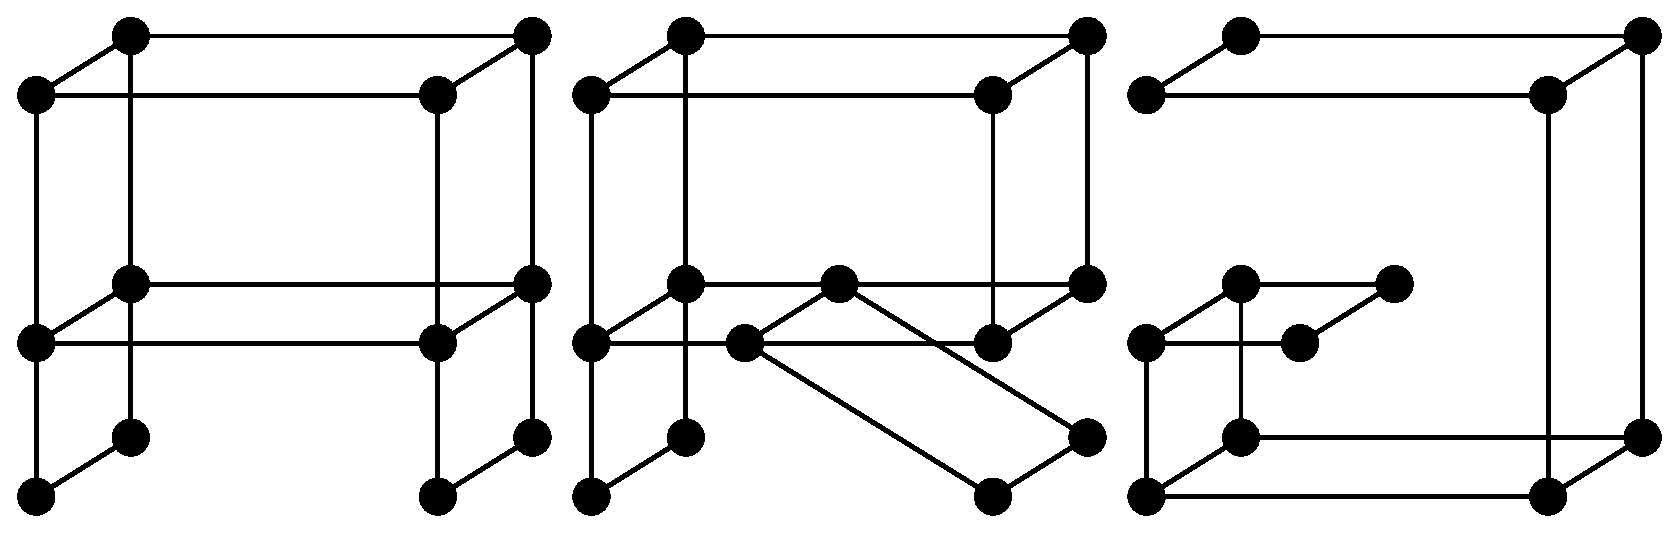
\epsfig{file=arg.eps,height=0.5in}\\%
     \normalsize\itshape Algorithms Research Group%
   }\hspace{0.7in}
   \protect\parbox[t]{2.2in}{%
     \noindent\centering%
     \epsfig{file=ufpr.eps,height=0.5in}\\%
     \normalsize Universidade Federal do Paraná%
   }\\[0.1in]
  \normalsize Mestrado em Ciência da Computação
}
\date{}

\renewcommand{\baselinestretch}{1.2}

\begin{document}

\maketitle

\tableofcontents

\section{Introdução}

\subsection{Básico}

\begin{Def}
  Uma \emph{\textit{hash}} é uma função $\funcao{h}{U}{M}$. $S\subseteq
  U$, $U=[0..u-1]$ finito, chamado de \emph{universo}. $M=[0..m-1]$
  finito.
  $\cardi{U}=u$, $\cardi{M}=m$, $\cardi{S}=n$. $x\in S$ é
  chamado de \emph{chave}. Cada $t\in M$ é chamado de
  \emph{endereço}. Uma tabela hash é uma área de armazenamento para as
  imagens dos elementos de $S$ por $h$. Se $h(x)=h(y)$, dizemos que $x$
  e $y$ são \emph{sinônimos} e dizemos que ocorreu uma
  \emph{colisão}. $h$ é \emph{perfeita} se é injetiva para os elementos
  de $S$. Se $h$ é perfeita e $m=n$, $h$ é \emph{mínima}. Particionamos
  $S$ em $\cj{S_0,\dotsc,S_{m-1}}$ onde
  \begin{equation*}
    S_i = \cjpp{x}{x\in S\we h(x) = i}\MMp
  \end{equation*}
\end{Def}

\subsection{FKS}

\begin{Teo}
  $m\geq n$. Então existe um $a\in [1..u-1]$ tal que, para
  $\funcaom{h}{x}{(ax\modu u)\modu m}$,
  \begin{equation*}
    \sum_{i=0}^{m-1}\binom{\cardi{S_i}}{2} = \frac{n(n-1)}{m}\MMp
  \end{equation*}
\end{Teo}

\begin{dem}
  $\binom{S_i}{2} = \cjpp{(x,y)}{x,y\in S, x\neq y, h(x)=h(y)=i}$. Se
  $x\neq y$ mas $h(x)=h(y)=i$, então
  \begin{equation*}
    (ax\modu u)\modu m = (ay\modu u)\modu m\MMp
  \end{equation*}
  Logo, $a(x-y)\modu u\in
  X=\cj{m,2m,3m,\dotsc,u-m,u-2m,u-3m,\dotsc}$. Portanto,
  \begin{equation*}
    \bigcup_a\bigcup_i\binom{S_i}{2}\simeq
    \bigcup_{x,y\in S\\x\neq y}\cjpp{a}{a(x-y)\modu u\in X}\MMv
  \end{equation*}
  e
  \begin{equation*}
    \begin{aligned}
      \sum_a\sum_i\binom{\cardi{S_i}}2 &=
      \sum_{\substack{x,y\in S\\x\neq y}}
      \cardi{\cjpp{a}{a(x-y)\modu u\in X}} \\
      &= \cardi{\cjpp{a}{\exists(x,y),x\neq y,a(x-y)\modu u\in X}}\MMp
    \end{aligned}
  \end{equation*}
  Como para todo $x,y$, $x\neq y$,
  $\cardi{\cjpp{a}{h(x)=h(y)}}<\frac{2u}m$,
  \begin{equation*}
    \sum_a\sum_i\binom{\cardi{S_i}}2 < \binom n2\frac{2u}m =
    \frac{un(n-1)}m\MMp
  \end{equation*}
  Logo, existe ao menos um $a$ tal que
  $\sum_i\binom{\cardi{S_i}}{2}<\frac{n(n-1)}m$.
\end{dem}

\begin{Cor}\label{soma3n}
  Existe um $a$ tal que, para $\funcaom{h}{x}{(ax\modu u)\modu n}$,
  $\sum_{i}\cardi{S_i}^2<3n$.
\end{Cor}

\begin{dem}
  Tomemos $m=n$, então $\sum_i\binom{\cardi{S_i}}{2}<n-1$. Como
  \begin{equation*}
    \cardi{S_i}^2 = 2\binom{\cardi{S_i}}{2}+\cardi{S_i}
  \end{equation*}
  e $\sum_i\cardi{S_i}=n$,
  \begin{equation*}
    \cardi{S_i}^2 = 2(n-1)+n<3n\MMp
  \end{equation*}
\end{dem}

\begin{Cor}\label{injetiva1-2}
  Existe $a$ tal que se $m=n(n-1)+1$, $h$ é injetiva para $S$.
\end{Cor}

\begin{dem}
  Existe um $a$ tal que
  \begin{equation*}
    \sum\cardi{S_i}^2 < \frac{2n(n-1)}{n(n-1)+1}+n < n+2\MMp
  \end{equation*}
  Como $\cardi{S_i}\in\MMN$ e como $\cardi{S_i}\leq 1$ --- supondo
  existir um $S_i$ tal que $\cardi{S_i}\geq 2$, temos que
  $\sum\cardi{S_i}^2\not< n+2$. Logo, $h$ injetiva para $S$.
\end{dem}

\begin{Def}[Esquema \emph{FKS}]
  Função de \hashing primária: $\funcaom{h}{x}{(ax\modu u)\modu n}$, onde
  $a$ é tal que $\sum\cardi{S_i}^2<3n$. A função primária fornece, para
  cada $x$, o
  índice $i$ para achar $a_i$ e $c_i$. As funções secundárias são as
  $\funcaom{h_1}{x}{(a_ix\modu
  u)\modu(\cardi{S_i}(\cardi{S_1}-1)+1)}$. $\cardi{S_i}(\cardi{S_1}-1)+1$
  é o $c_i$, que é o tamanho da tabela \textit{hash} para $h_i$. As
  chaves $x$ são armazenadas na tabela $D$ em $C_i+h_i(x)$, onde os
  $C_i=\sum_{j=0}^{i=1}c_j$ são também previamente armazenados numa
  tabela $C$, assim como os $a_i$ em $A$ e os $c_i$ em $c$. A \hashing é
  feita por $h_i\circ h$. Note que $(h_i\circ
  h)(x)=C_i+h_i(x)$. $h_i\circ h$ requer $a$, $u$, $n$, $A[0..n-1]$,
  $c[0..n-1]$, $C[0..n-1]$. Total de $3n+O(1)$ locações, ou
  $(3n+O(1))\log u$ bits. Assim $D$ também requer $3n\log u$
  bits. Porém, gostaríamos de $\Omega(n+\log\log u)$ bits. Ademais,
  construir a representação de $S$ pode ser $O(nu)$ no pior caso ---
  para encontrar $a$, podemos ter de fazer uma busca exaustiva que
  custaria $O(nu)$: $u$ possibilidades testado os $n$ elementos de $S$
  cada.
\end{Def}

\subsection{FKS um pouco melhorado}

\begin{Cor}
  Para pelo menos metade dos valores $a\in[1..u-1]$,
  $\sum_{i=0}^{n-1}\cardi{S_i}^2 < 5n$.
\end{Cor}

\begin{dem}
  Como
  \begin{equation*}
    \sum_{a=1}^{u-1}\sum_{i=0}^{m-1}%
    \binom{\cardi{S_i}}{2}<\frac{un(n-1)}{m}\MMv
  \end{equation*}
  Se $m=n$,
  \begin{equation*}
    \sum_{a=1}^{u-1}\sum_{i=0}^{m-1}%
    \binom{\cardi{S_i}}{2}< u(n-1) = u(m-1)\MMp
  \end{equation*}
  Logo,
  \begin{equation*}
    \sum_{a=1}^{u-1}\biggl(\sum_{i=0}^{m-1}%
    \cardi{S_i}^2-n\biggr) < 2u(n-1)\MMp
  \end{equation*}
  Já que, para todo $a$, $\sum_{i=0}^{m-1}%
  \cardi{S_i}^2-n\geq 0$, portanto só para no máximo metade dos $a$ pode
  ocorrer
  \begin{equation*}
    \sum_{i=0}^{m-1}%
    \cardi{S_i}^2-n\geq 2(2(n-1))\MMpv
  \end{equation*}
  ou seja, só para no máximo metade dos $a$ pode ocorrer de a soma
  exceder o dobro da média. Logo, para no mínimo metade dos $a$,
  \begin{equation*}
    \sum_{i=0}^{m-1}%
    \cardi{S_i}^2-n< 4(n-1)\MMp
  \end{equation*}
\end{dem}

\begin{Cor}\label{metadeinjetiva}
  Para no mínimo metade dos $a$, $\funcaom{h}{x}{(ax\modu
    u)\modu(2n(n-1)+1)}$ opera injetivamente em $S$.
\end{Cor}

\begin{dem}
  $m=2n(n-1)+1$,
  \begin{equation*}
    \sum\biggl(\sum\cardi{S_i}-n\biggr) <
    \frac{2un(n-1)}{2n(n-1)+1}<u\MMp
  \end{equation*}
  Logo, para no máximo metade dos $a$ a soma pode exceder $2$. Logo,
  para
  no
  mínimo metade dos $a$ a soma é menor que $2$.
\end{dem}

\begin{Def}[FKS melhorado]
  Agora, $a$ e $a_i$ são escolhidos aleatoriamente até serem
  apropriados. Como a probabilidade de $a$ ou de algum $a_i$ tomado
  aleatoriamente ser apropriado é maior que $\frac12$, o número esperado
  de sorteios para se encontrar um $a$ ou um $a_i$ apropriado é no
  máximo $2$. Assim, para achar $a$ e todos os $a_i$ em $[0,n-1]$,
  gasta-se $O(n)$. Para a tabela $D$, precisamos de
  $\sum_{i=0}^{n-1}(2\cardi{S_i}(\cardi{S_i}-1)+1) =
  2\sum\cardi{S_i}^2-n = 9n\log u$ bits.
\end{Def}

\subsection{Mais um melhoramento}

\begin{Teo}
  Existe um primo $q<n^2\log u$ tal que $\funcaom{\zeta}{x}{x\modu q}$ é
  perfeita para $S$.
\end{Teo}

\begin{dem}
  $S=\cj{x_1,\dotsc,x_n}$. Note que $i\neq j$ implica $x_i\neq x_j$ e
  $x_i-x_j\neq 0$. Seja $t=\prod_{i<j}(x_i-x_j)\prod_ix_i$. É claro que
  $|t|\leq u^{\binom{n+1}{2}}$ e, portanto, $\log|t|\leq\binom{n+1}2\log
  u$. Do teorema dos números primos, para um $x$,
  \begin{equation*}
    \log\biggl(\prod_{\substack{q<x\\q\text{ primo}}}q\biggr) = x+o(x)\MMp
  \end{equation*}
  Supondo que $q$ divide $t$ para todo primo $q<n^2\log u$, temos
  \begin{equation*}
    n^2\log u+o(n^2\log u)<\binom{n+1}2\log u\MMv
  \end{equation*}
  o que é um absurdo. Logo, existe um $q<n^2\log u$ tal que $q$ não
  divide $t$. Portanto, para esse $q$, $\zeta$ é perfeita.
\end{dem}

\begin{Def}[Melhoramento do esquema FKS]
  Como o pior caso para representar $S$ é $O(nu)$, se $u<n^2\log u$,
  $O(nu)=O(n^2\log u)$. Se $u\geq n^2\log u$, computamos um primo $q$
  que dá $\zeta$ perfeita. Encontrar o primo é $O(nq)=O(n^3\log
  u)$. Agora, não usamos mais $x$, mas $\zeta(x)$ no lugar. Trocamos o
  universo $[0,u-1]$ por $[0,q-1]$, para $q<n^2\log u$. Representar $S$
  leva tempo de construção $O(n^3\log u)$ deterministicamente. Dessa
  vez, a função \textit{hash} é $h_i\circ h\circ\zeta$. O esquema, cujo
  espaço de representação queremos que seja $O(n\log n+\log\log u)$, é o
  seguinte:
  \begin{enumerate}
  \item $\funcao{\rho}{S}{[0..n^2-1]}$,
    $\funcaom{\rho}{x}{(a_{\rho}x\modu q)\modu n^2}$ tal que
    $a_{\rho}<q<n^2\log u$ e $S'=\rho(S)$.
  \item A \hashing primária é $\funcao{h}{S'}{[0..n-1]}$,
    $\funcaom{h}{x}{(ax\modu p)\modu n}$, que conseguimos por causa do
    corolário~\ref{soma3n}. $p > n^2-1$, $a\in[1,p-1]$,
    $\sum\cardi{S_i}^2<3n$.
  \item $\funcao{h_i}{S_i}{[0..c_i-1]}$,
    $c_i=\cardi{S_i}(\cardi{S_i}-1)+1$. $\funcaom{h_i}{x}{(a_ix\modu
      p)\modu c_i}$, $a_i\in[1..p-1]$, do corolário~\ref{injetiva1-2}. O
    esquema é $x\in S$ ir para $t_i=C_i+h_i(\rho(x))$ numa tabela de
    chaves de tamanho $3n\log u$ bits $P[0..3n-1]$, ou melhor, $3n\log
    n$ bits. $t_i$ fornece o índice para a tabela $D[0..n-1]$, que
    requer só $n\log u$.
\end{enumerate}
$a_{\rho}$ e $q$ requeremm $2\log n+\log\log u$ bits cada. Para a função
$h$, $a$ e $p$ requerem $4\log n$ bits. Para as $h_i$, precisamos de
tabelas $A[0..n-1]$ para os $a_i$, $c[0..n-1]$ para os $c_i$ e
$C[0..n-1]$ para os $C_i$: total $3n\log n$. $P$ também precisa de
$3n\log n$. O total é $6n\log n+8\log n+2\log\log u=O(n\log n+\log\log
u)$, além dos $n\log u$ bits de $D$. O tempo e construção do esquema é
$O(n^3\log u)$, mas a busca é $O(1)$.
\end{Def}

\begin{Ex}
  Seja
  $S_X=\cj{\text{\texttt{JAN}},\text{\texttt{FEB}},
    \text{\texttt{MAR}},\text{\texttt{APR}},\dotsc,
    \text{\texttt{DEC}}}$ e
  \begin{equation*}
    S=\cj{217=\text{\texttt{`J'}}+\text{\texttt{`A'}}+
    \text{\texttt{`N'}},\dotsc,204=\text{\texttt{`D'}}+
    \text{\texttt{`E'}}+\text{\texttt{`C'}}}
  \end{equation*}
  (considerando a
  codificação
  ASCII).
  $\funcaom{\rho}{x}{(14x\modu 167)\modu 144}$.
  $S\mapsto S'=\cj{14,\dotsc,120}$. $\funcaom{h}{x}{(4x\modu 149)\modu
    12}$
  particiona $S'$ em $S_0,\dotsc,S_{11}$. Encontramos os
  $\funcaom{h_i}{x}{(a_ix\modu 149)\modu c_i}$. Note que
  $S_3=S_6=\emptyset$.

  \begin{center}
    \begin{tabular}{c|cccccccccccc}
      $i$ & $0$ & $1$ & $2$ & $3$ & $4$ & $5$ & $6$ & $7$ & $8$ & $9$ &
      $10$ & $11$ \\
      \hline
      $a_i$ & $1$ & $1$ & $1$ & & $1$ & $2$ & & $1$ & $1$ & $1$ &
      $1$ & $2$ \\
      $c_i$ & $1$ & $1$ & $1$ & & $1$ & $3$ & & $1$ & $1$ & $1$ &
      $1$ & $3$
    \end{tabular}
  \end{center}
\end{Ex}

\subsection{Schmidt e Siegel}

\begin{Lem}\label{lemlogaritmico}
  Sejam $S_j$, $j\in[t]$, subconjuntos disjuntos de $U$, $\cardi{U}=u$ e
  $t\leq u$. Então, existe um $a\in U$ para o qual qualquer
  $\funcao{h_j}{U}{M}$, $\funcaom{h_j}{x}{(ax\modu u)\modu c_j}$,
  $c_j=2\cardi{S_i}(\cardi{S_i}-1)+1$, opera injetivamente em metade dos
  $S_j$.
\end{Lem}

\begin{dem}
  Dado um $a$, existe colisão entre $x$ e $y$ se $x\neq y$ mas
  $h_j(x)=h_j(y)=k$, para algum $k\in[0..c_j-1]$, ou seja, se
  \begin{equation*}
    (ax\modu u)\modu c_j = (ay\modu u)\modu c_j\MMp
  \end{equation*}
  Portanto, $a(x-y)\modu u\in
  X_1=\cj{c_j,2c_j,3c_j,\dotsc,u-c_j,u-2c_j,u-3c_j,\dotsc}$. Assim,
  \begin{equation*}
    \begin{aligned}
      \sum_{a=1}^{u-1}\sum_{j=1}^t\sum_{k=0}^{c_j-1}
      \cardi{\cjpp{(x,y)}{x,y\in S_j,x\neq y,h_j(x)=h_j(y)=k}} \\
      = \sum_{j=1}^t\sum_{a=1}^{u-1}\sum_{k=0}^{c_j-1}
      \cardi{\cjpp{(x,y)}{x,y\in S_j,x\neq y,h_j(x)=h_j(y)=k}} \\
      = \sum_{j=1}^t\sum_{\substack{x,y\in S_j\\x\neq y}}
      \cardi{\cjpp{a}{a(x-y)\modu u\in X_1}} \\
      < \frac{2u\binom{\cardi{S_j}}{2}}{2\cardi{S_j}(\cardi{S_j}-1)+1}
      < \frac{ut}2\MMp
    \end{aligned}
  \end{equation*}
  Logo, para pelo menos um dos $u-1$ possíveis
  $a$ é preciso não haver colisões para
  menos $\frac{t}2$ conjuntos $S_j$.
\end{dem}

\begin{Def}[Esquema FKS de Schmidt e Siegel]
  Usa uma função \textit{hash} composta $h_z\circ h\circ\rho$ como
  descrita anteriormente, mas:
  \begin{enumerate}[(a)]
  \item o espaço para cada \textit{bucket} de colisão $S_i$ é
    $c_i=2\cardi{S_i}(\cardi{S_i}-1)+1$;
  \item são guardados apenas $\chao{\log n}+1$ multiplicadores $a_z$
    para a função \hashing secundária --- isso porque, do
    lema~\ref{lemlogaritmico}, existe um $a_0$ para o qual ${h_i}_0$
    opera injetivamente para pelo menos metade dos $S_i$. Para a metade
    restante, existe um $a_1$ para o qual ${h_i}_1$ opera injetivamente
    para pelo menos metade dessa metade restante. E, assim por diante,
    até um $a_z$ que serve cerca de $\frac{1}{2^{z+1}}$ dos $S_i$.
  \end{enumerate}
  A grande sacada agora é como representar as tabelas $A$, $c$, $C$ e
  $P$ em espaço $O(n)$ e ainda manter a busca $O(1)$.

  Para montar $C$ contendo os $C_i=\sum_{j=0}^{i-1}c_j=
  \sum{j=0}^{i-1}(2\cardi{S_j^h}(\cardi{S_j^h}-1)+1)$, seja $\chi_j$ a
  \textit{string} unária de $c_j$ $1$'s que codificamm $c_j$. As
  \textit{strings}
  $\chi_j$ são guardadas numa tabela $T_0$, com um $0$ separando duas
  \textit{strings} consecutivas. Como cada $\chi_j$ requer exatamente
  $c_j$ bits, temos, pelo corolário~\ref{soma3n}, que o tamanho de $T_0$
  é
  \begin{equation*}
    \sum_{j=0}^{n-1}(\cardi{\chi_j}+1) = \sum_{j=0}^{n-1}c_j + n \leq 4n
  \end{equation*}
  bits. Assumamos então que $T_0$ é guardado como uma sequencia de
  palavras
  de tamanho $\teto{\log(4n)}$ bits. Sabemos que extrair uma
  subsequencia de bits de uma palavra de tamanho $O(\log n)$ bits é algo
  que pode ser executado em tempo constante, assim como concatenar duas
  \textit{strings} de tamanhos $O(\log n)$ bits. Logo, cada bit em $T_0$
  é endereçável.

  Dividimos as $n$ \textit{strings} codificadas em $T_0$ em
  $\teto{\frac{n}{\teto{\log n}}}$ grupos de $\teto{\log n}$ strings
  cada, com a possível exceção do último grupo. Seja $\lambda_i$,
  $0\leq\lambda_i<4n$, o endereço (índice) do bit inicial da primeira
  \textit{string} do $i$-ésimo grupo, ou seja, a \textit{string}
  $\chi_{i\teto{\log n}}$, sendo $i\in[0..\teto{\frac{n}{\teto{\log
        n}}}-1$.

  Analogamente, construímos uma tabela $T_1$ contendo os $\lambda_i$,
  sendo
  $i\in[1..\teto{\frac{n}{\teto{\log n}}}]$, em binário, armazenados
  como palavras de $\teto{\log(4n)}$ bits. Note que $\lambda_0=0$ não é
  armazenado. O tamanho da tabela $T_1$ é $\teto{\frac{n}{\teto{\log
        n}}}\teto{\log(4n)}=O(n)$ bits. Notemos ainda que
  \begin{equation*}
    \lambda_i=C_{i\teto{\log n}}+i\teto{\log n}\MMp
  \end{equation*}
  Logo, podemos utilizar $\lambda_i$ para obter $C_{i\teto{\log
      n}}$. Assim como extrair uma subsequência de bits de uma palavra
  de tamanho $O(\log n)$ bits pode ser feito em tempo constante, acessar
  algumas (um número constante de)
  constantes de uma palavra de tamanho $O(\log n)$ também pode ser feito
  em tempo constante. Se $\lambda_{i+1}-\lambda_i\leq
  2\teto{\log(4n)}$, os endereços dos $c_j$ intermediários, para
  $i\teto{\log n}\leq j<(i+1)\teto{\log n}$, que nos permitem computar
  os $C_j$ correspondentes, podem ser codificados em tempo $O(1)$
  através de acessos às tabelas $T_0$ e $T_1$. Se, entretanto,
  $\lambda_{i+1}-\lambda_i>\teto{\log(4n)}^2$, usamos a tabela $T_2$.

  A tabela $T_2$ armazena, começando no bit inicial pertinente a
  $\lambda_i$, $\teto{\log n}-1$ índices binários para os pontos
  iniciais dos $\chi_j$ em $T_0$, sendo $i\teto{\log
    n}<j<(i+1)\teto{\log n}$.

  Agora, se
  $2\teto{\log(4n)}<\lambda_{i+1}-\lambda_i\leq\teto{\log(4n)}^2$,
  procedemos da seguinte maneira. Especialmente, cada grupo de
  \textit{strings} é dividido em $\teto{\frac{\teto{\log
        n}}{\teto{\log\log n}}}$ subgrupos, cada um com $\teto{\log\log
    n}$ \textit{strings}. Denote por $\eta_{i,j}$ o endereço de $T_0$ do
  ponto inicial de $\chi_{i\teto{\log n}+j\teto{\log\log n}}$, para
  $j\in[1..\teto{\frac{\teto{\log n}}{\teto{\log\log n}}}-1]$. Assim,
  $\lambda_i<\eta_{i,j}<\lambda_{i+1}$. Os \textit{offsets} binários
  $\eta_{i,1}-\lambda_i$, $\eta_{i,2}-\lambda_i$ etc. são armazenados em
  $T_2$
  como
  números de $2\teto{\log\log(4n)}$ bits começando pelo local
  $\lambda_i$. Se $\eta_{i,j+1}-\eta_{i,j}\leq 2\teto{\log(4n)}$, a
  informação
  para o $c_k$ intermediário, $i\teto{\log n}+j\teto{\log\log n}<k<
  i\teto{\log n}+(j+1)\teto{\log\log n}$, pode ser facilmente
  decodificada da tabela $T_0$. Caso contrário, os \textit{offsets} de
  tamanho $2\teto{\log\log(4n)}$ de todos os $c_k$ intermediários são
  armazenados numa tabela $T_3$ de $4n$ bits, começando com o ponto
  pertinente a $\eta_{i,j}$. Essa última codificação requer
  $(\teto{\log\log n}-1)\cdot 2\teto{\log\log(4n)}\leq 2\teto{\log(4n)}$
  bits.
\end{Def}

\begin{Ex}
  Para $S=\cj{2,4,5,15,18,30}$, $n=6$, $u=31$, codificamos a tabela $C$
  da seguinte maneira. Os valores $c_0=1$, $c_1=0$, $c_2=1$, $c_3=0$,
  $c_4=3$ e $c_5=3$ são armazenados em unário na tabela $T_0$ de tamanho
  $4n=24$ bits. As \textit{strings} de codificação são divididas em
  $\teto{\frac{n}{\teto{\log n}}}=\teto{\frac{6}{\teto{\log 6}}}=2$
  grupos de $\teto{\log n}=\teto{\log 6} = 3$ \textit{strings} cada. A
  tabela $T_i$ contém os índices $\lambda_i$, $i\in\cj{1,2}$, para os
  pontos iniciais das \textit{strings} $\chi_3$ e $\chi_6$ em $T_0$. Já
  que tanto $\lambda_1-\lambda_0$ quanto $\lambda_2-\lambda_1$ são no
  máximo $2\teto{\log(24)}=10$, nenhum nível adicional é necessário.
\end{Ex}

É fácil ver que não é mais necessário guardar os valores $c_i$, pois
eles podem ser encontrados em tempo constante através da representação
de $C$ como descrita acima.

As tabelas $P$ e $A$ podem ser codificadas de uma maneira similar. Em
particular, os $a_0,a_1,\dotsc,a_{\chao{\log n}}$ (lembrar do
lema~\ref{lemlogaritmico})
são guardados em um
\textit{array} de $\chao{\log n}+1$ palavras. Total: $O((\log n)^2)$
bits. A tabela $A_0$ contém $n$ \textit{strings} em unário que codificam
os índices dos multiplicadores associados a cada \textit{bucket} de
colisão. A $i$-ésima sequência de bits codifica o inteiro
$j_i\leq\teto{\log n}$ se $a_{j_i}$ é o multiplicador associado ao
\textit{bucket} $S_i$. O primeiro multiplicador codificado pela
\textit{string} $0$ é usável para pelo menos metade dos
\textit{buckets}. O segundo multiplicador, codificado pela
\textit{string} $10$ é usável para pelo menos $\frac14$ dos
\textit{buckets} etc. Desse modo, a sequência de bits em $A_0$ contempla
no máximo $\frac n2$ $0$'s, $\frac n4$ $10$'s etc. Total do tamanho da
\textit{string} é no máximo $2n$ bits. Logo, pode-se encontrar o
multiplicador associado a cada \textit{bucket} em tempo $O(1)$.

Finalmente, a complexidade do espaço do esquema de Schmidt e Siegel é
$O(n+\log\log u)$. O esquema requer $O(n)$ bits para codificar os
\textit{offsets} $C_i$, a tabela $P$ e os multiplicadores $a_j$, além de
$O(2\log n+\log\log u)$ bits para armazenar os parâmetros $a_{\rho}$ e
$q$ da função de pré-processamento. Assim, temos o seguinte teorema.

\begin{Teo}[Schmidt e Siegel]\footnote{Nota: a prova deste teorema não
    está escrita explicitamente, embora muito dela tenha sido feito nos
    comentários anteriores. Depois eu pretendo arrumar isso.}
  Para um conjunto $S$ de $n$ elementos de um universo
  $U=\cj{0,\dotsc,u-1}$, existe uma função \textit{hash} perfeita de
  tempo constante com complexidade de espaço $\Theta(n+\log\log u)$.
\end{Teo}

\section{Hashing perfeita probabilística}

\subsection{O melhoramento do FKS de Dietzfelbinger}

\begin{Def}[Dietzfelbinger]
  Seja $\Hdie^d=\cjpp{h_a}{a=(a_0,a_1\dotsc,a_d)\in U^{d+1}}$ em que
  \begin{equation*}
    \funcaom{h_a}{x}{\biggl(\sum_{i=0}^da_ix^i\biggr)\modu u}\MMp
  \end{equation*}
  Seja $\funcao{\zeta}{U}{M}$, $\funcaom{\zeta}{x}{x\modu
    m}$. $\Hdie^d_m=\cjpp{\zeta\circ g}{g\in \Hdie^d}$. Para todo
  $h\in\Hdie^d_m$ definimos $S^h_i=h^{-1}(i)\cap S$, $i\in M$, e
  $B^h_k=\sum_{i\in M}\binom{\cardi{S^h_i}}{k}$.
\end{Def}

\begin{Teo}\label{teoHdie}\footnote{Nota: a prova deste teorema não é
    apresentada no artigo, apenas referenciada.
    Eu pretendo, no futuro, buscá-la nas referências e
    acompanhá-la. Mas, ainda não o fiz.}
  Para um $S\subseteq U$ fixo e um $h\in \Hdie^d_m$ aleatório, $d\geq
  3$, $B^h_2<\frac{3\cardi{S}^2}m$ com probabilidade
  $1-O(\Bigl({\frac{\cardi{S}^2}m}\Bigr)^{-\epsilon})$ para algum
  $\epsilon>0$.
\end{Teo}

O teorema acima é usado para mostrar como o FKS pode ser rodado em tempo
linear com probabilidade alta.
\begin{enumerate}
  \item Tome uma $h$ aleatoriamente de
    $\Hdie^3_m$, com $m=n=\cardi{S}$. Do teorema~\ref{teoHdie}, $h$ é
    boa com probabilidade
    $1-O(\Bigl({\frac{\cardi{S}^2}m}\Bigr)^{-\epsilon})=1-O(n^{-1})$. Portanto,
    este primeiro passo termina em tempo $O(n)$ com probabilidade
    $1-O(n^{-1})$.
  \item Para cada \textit{bucket} $S^h_i$ tome aleatoriamente uma função
    $h_i$ de $\Hdie^{1,1}_{2\cardi{S_i}^2}$. Seja $t_i$ a variável
    aleatória que representa o número de tentativas necessárias para ser
    enncontrada uma $h_i$ apropriada. Do
    corolário~\ref{metadeinjetiva}, $\MMP[t_i=1]\geq\frac12$ e,
    consequentemente, $\MME(t_i)\leq 2$ e $\Var(t_i)\leq 2$. Se $T_i$ é
    o número de operação necessárias para encontrar $h_i$ apropriada,
    então $T_i=O(t_i\cardi{S_i})$, $\MME(T_i)=O(\cardi{S_i})$ e
    $\Var(T_i)=O(\cardi{S_i}^2)$. Tomemos $T=\sum_{i\in M}T_i$. Como as
    escolhas $h_i$ são independentes, $E(T)=\sum_{i\in
      M}O(\cardi{S_i})=O(n)$ --- como queríamos --- e
    $\Var(T)=\sum_{i\in M}O(\cardi{S_i}^2)=O(n)$. Portanto, da
    desigualdade de Chebyshev segue que este segundo passo também
    termina com $T=O(n)$ com probabilidade $1-O(n^{-1})$.
\end{enumerate}

\subsection{Dietzfelbinger e Meyer auf der Heide}

\begin{Def}
  Sendo $r,m\geq 1$, $d_1,d_2\geq 1$, $f\in\Hdie^{d_1}_r$,
  $g\in\Hdie^{d_2}_m$, $a_1,\dotsc,a_r\in[m]$ e
  $h=h(f,g,a_1,\dotsc,a_r)$ definida como, para $x\in U$,
  \begin{equation*}
    h(x) = (g(x)+a_{f(x)})\modu m\MMv
  \end{equation*}
  definimos
  \begin{equation*}
    \Rdie(r,m,d_1,d_2)=
    \cjbar{\funcao{h}{U}{[m]}}{h=h(f,g,a_1,\dotsc,a_r)}\MMp
  \end{equation*}
  Convencionamos que $h(f,g,a_1,\dotsc,a_r)$ e
  $h(f',g',a'_1,\dotsc,a'_r)$ são diferentes quando
  $(f,g,a_1,\dotsc,a_r)$ e $(f',g',a'_1,\dotsc,a'_r)$ são diferentes,
  mesmo que  sejam extensionalmente iguais
  $h(f,g,a_1,\dotsc,a_r)$ e
  $h(f',g',a'_1,\dotsc,a'_r)$.
\end{Def}

Se $m=n$, $r=n^{1-\delta}$ para algum $\delta>0$, $\Rdie(r,m,d_1,d_2)$
pode ser explicada como a seguir. A função $f\in\Hdie^{d_1}_r$
particiona $S$ em $r$ \textit{buckets} $S^f_i=f^{-1}(i)\cap S$, $0\leq
i<r$. Entretanto, ao invés de, como no esquema FKS, mapear as chaves do
\textit{bucket} $S^f_i$ em um único espaço de tamanho
$2|S^f_i|^2$, aplicaremos uma segunda função \textit{hash}:
$g(x)+a_i$, com todos os \textit{buckets} compartilhando o alcance comum
$[1,m]$.

\begin{Teo}[Dietzfelbinger e Meyer auf der
  Heide]\label{DMADH}\footnote{Nota: a prova deste teorema não é
    apresentada no artigo, apenas referenciada.
    Eu pretendo, no futuro, buscá-la nas referências e
    acompanhá-la. Mas, ainda não o fiz.}
  Tomando um $0<\delta<1$ fixo e $r=n^{1-\delta}$ e escolhendo
  aleatoriamente
  $f\in\Hdie^d_r$,
  \begin{equation*}
    \MMP[|S^f_i|\leq 2n^\delta\text{ para todo $i$}]\geq
    1-O(n^{1-\delta-\frac{\delta d}{2}})\MMp
  \end{equation*}
\end{Teo}

Isso significa que com $r=n^{1-\delta}$ e
$d_1>\frac{2(1-\delta)}{\delta}$ temos alta probabilidade de todos os
\textit{buckets} terem tamanho próximo da média, que é
$n^{\delta}$. Para um $d_2$ suficientemente grande e $m=O(n)$, a segunda
função \textit{hash} $G$ mapeia cada $x\in S^f_i$ para um único
endereço, novamente com alta probabilidade.

\subsection{FKS com grafos aleatórios} % pág. 98

Podemos enxergar o método FKS como um mapeamento de $S$ para uma
floresta de estrelas de núcleos ``pequenos''. Uma estrela é uma árvore
onde todos os vértices, com exceção do núcleo, têm grau $1$. A função
primária $h$ mapeia cada $x$ no núcleo de uma estrela do grafo (a
floresta de estrelas). A função secundária $h_i$ mapeia o núcleo para um
de seus vizinhos.

\begin{Probl}[Problema da associação perfeita (Czech)]
  Dado um $G=(V,E)$, $|V|=\nu$ e $|E|=\mu$, encontrar uma função
  $\funcao{g}{V}{[0..\mu-1]}$ tal que $\funcao{h}{E}{[0..\mu-1]}$
  definida como
  \begin{equation*}
    h(e=\cj{a,b}) = (g(a)+g(b))\modu \mu
  \end{equation*}
  é uma bijeção.
\end{Probl}

Para um grafo acíclico, a solução para esse problema é um procedimento
simples em tempo ótimo:
\begin{enumerate}
\item Distribua os $h(e)=0,\dotsc,\mu-1$ para as arestas $e$
  em qualquer ordem.
\item Para cada componente conexa de $G$ escolha um vértice $v$ e
  atribua $g(v)=0$ e:
  \begin{enumerate}
  \item Faça uma busca em profundida no grafo.
  \item Para cada vértice $b$ alcançado por um vértice $a$ (tal que o
    valor associado a $e=\cj{a,b}$ é $h(e)$), atribua
    $g(b)=(h(e)-g(a))\modu\mu$.
  \end{enumerate}
\end{enumerate}

Agora, para encontrar a $f$ que associa os $x$ às estrelas, procedemos
do seguinte modo (chamado de ``fase de mapeamento''):
\begin{enumerate}
\item Escolha duas funções \textit{hash} independentes aleatoriamente,
  $f_1$ e $f_2$, de domínio $U$ e contradomínio $[0..\nu-1]$.
\item Para cada $x\in S$,
  se $f_1(x)=f_2(x)$, modifique $f_2(x)$ acrescentando um número
  aleatório em $[1..\nu-1]$ (isso para evitar \textit{loops});
\item $S$ agora está correspondido com um grafo
  \begin{equation*}
    G=(V=[0..\nu],E=\cjpp{\cj{f_1(x),f_2(x)}}{x\in S})\MMp
  \end{equation*}
  Então, testa
  se $G$ é acíclico. Senão, joga fora $f_1$ e $f_2$ e pega outras até
  ter $G$ acíclico.
\end{enumerate}

Observe que sortear as $f_1$ e $f_2$ é rápido. Testar se $G$ é acíclico
também é rápido. Ademais, a quantidade de grafos acíclicos é grande no
espaço amostral. Se $f_1$ e $f_2$ são computáveis em tempo $O(1)$, gerar
o grafo $G$ correspondente é $O(\mu)$ (busca) e verificar se ele é
acíclico é $O(\nu+\mu)$.

Estratégia: precisamos ter $\mu=n=|S|$ e $\nu=O(\mu)$. Verificar essas
duas condições leva tempo similar. Porém, para $\nu=c\mu$, para alguma
constante $c$, a probabilidade um grafo aleatório ser acíclico continua
grande o suficiente? Nessas novas condições, os grafos acíclicos dominam
o espaço de todos os grafos aleatórios?

\begin{Teo}[Havas]\label{TeoHavas}
  Seja $G$ um grafo aleatório com $\nu$ vértices e $\mu$ arestas obtido
  escolhendo aleatória e independentemente as $\mu$ arestas com
  repetição. Então, se $\nu=c\mu$ para $c>2$, a probabilidade de $G$ ser
  acíclico, quando $\nu\tende\infty$, é
  \begin{equation*}
    p = \MMe^{\frac1c}\sqrt{\frac{c-2}{c}}\MMp
  \end{equation*}
\end{Teo}

\begin{dem}
  Erdös e Rényi mostraram\footnote{No futuro, também esta é uma
    demonstração que eu pretendo acompanhar.}
  que a probabilidade de um grafo aleatório não
  ter ciclos, à medida que $\nu=c\mu$ tende ao infinito, é
  \begin{equation*}
    \MMe^{\frac{1}{c}+\frac{1}{c^2}}\sqrt{\frac{c-2}{c}}\MMp
  \end{equation*}
  Porém, em nosso caso, os grafos gerados no passo de mapeamento podem
  ter arestas múltiplas (não \textit{loops}). A probabilidade procurada
  $p$, então, é a probabilidade calculada por Erdös e Rényi vezes a
  probabilidade de não haverem arestas múltiplas. Sabemos que a
  $j$-ésima aresta é única com probabilidade
  \begin{equation*}
    \frac{\binom{\nu}{2}-j+1}{\binom{\nu}{2}}\MMp
  \end{equation*}
  Logo, a probabilidade de todas as arestas serem únicas é
  \begin{equation*}
    \prod_{j=1}^{\mu}\frac{\binom{\nu}{2}-j+1}{\binom{\nu}{2}}
    = \MMe^{-\frac{-1}{c^2}+o(1)}
  \end{equation*}
  Finalmente,
  $p=\biggl(\MMe^{\frac{1}{c}+\frac{1}{c^2}}\sqrt{\frac{c-2}{c}}\biggr)
  \biggl(\MMe^{-\frac{-1}{c^2}+o(1)}\biggr)=
  \MMe^{\frac1c}\sqrt{\frac{c-2}{c}}$.
\end{dem}

O algoritmo é realmente bem eficiente. Para uma constante $c$ tão
pequena quanto $2,09$, por exemplo, o número esperado de execuções (de
tentativas para $G$) é menor (estritamente) que $3$.

\begin{Ex}
  $S=\cj{53,59,61,67,71,73,79,83,89,97}$ o conjunto de todos os primos
  maiores que $50$ e menores que $100$. Encontramos o acíclico $G$ com
  as funções:
  \begin{equation*}
    \begin{aligned}
      f_1(x) &= ((34x+11)\modu 101)\modu 21; \\
      f_2(x) &= ((29x+18)\modu 101)\modu 21.
    \end{aligned}
  \end{equation*}
  Sortear uma função dessas é sortear os coeficientes $a_1$ e $a_0$ no
  conjunto $[1..101-1]$. Assim, a correspondência entre $S$ e $G$ fica
  como na tabela abaixo:
  \begin{center}
    \begin{tabular}{cccccccccc}
      $53$ & $59$ & $61$ & $67$ & $71$ & $73$ & $79$ & $83$ & $89$ &
      $97$ \\\hline
      $\cj{12,19}$ & $\cj{12,14}$ & $\cj{2,7}$ & $\cj{4,0}$ &
      $\cj{1,15}$ &
      $\cj{14,6}$ & $\cj{8,3}$ & $\cj{5,1}$ & $\cj{7,11}$ &
      $\cj{3,14}$\\
    \end{tabular}
  \end{center}

  Decidimos armazenar o $i$-ésimo primo na
  $(i-1)$-ésima posição. Ex: $83$, o $8$\upo primo, recebe endereço
  $7$. Ou seja, $h(\cj{5,1})=7$. No segundo passo, considerando uma
  componente conexa de cada vez, resolvemos o problema da associação
  perfeita valorando os $g$. Para checar se $59$ é primo, computamos
  $f_1(59)=14$ e $f_2(59)=12$. Depois, $h(\cj{14,12})=1$. Checando o
  endereço $1$ na tabela, confirmamos que $59$ é primo.
\end{Ex}

\subsection{Métodos com hipergrafos}

\begin{Probl}[Problema da associação perfeita para hipergrafos]
  Dado um $r$-hipergrafo $G=(V,E)$ em que $E\subseteq\binom{V}{r}$ e
  $\cardi{V}=\nu$ e $\cardi{E}=\mu$, encontrar uma função
  $\funcao{g}{V}{[0..\mu-1]}$ tal que, para $\funcao{h}{E}{[0..\mu-1]}$
  definida como
  \begin{equation*}
    h(e=\cj{v_1,\dotsc,v_r}) = (g(v_1)+\dotsb+g(v_r))\modu \mu
  \end{equation*}
  é uma bijeção.
\end{Probl}

Do mesmo modo que com $2$-hipergrafos, somente $r$-hipergrafos acíclicos
têm a garantia de ter uma solução em tempo linear para o problema da
associação perfeita.

\begin{Def}
  Um $r$-hipergrafo é \emph{acíclico} se não contém subgrafo com grau
  mínimo $2$.
\end{Def}

Outra definição equivalente:

\begin{Def}
  Um $r$-hipergrafo é \emph{acíclico} se e só se há algum modo de
  retirar sucessivamente arestas contendo vértices de grau $1$ e, no
  final, ficar com um grafo sem arestas.
\end{Def}

Então, para verificarmos se um hipergrafo é acíclico, faremos o
seguinte:
\begin{enumerate}
\item Inicialmente, marque todas as arestas como ``não removidas''.
\item Visite todos os vértices do grafo, cada vértice apenas uma vez:
  \begin{enumerate}
  \item Se $v$ tem grau $1$, remova do grafo a aresta $e$ que levou a
    $v$.
  \item Cheque se algum dos outros vértices da aresta removida possui
    grau $1$. Se sim para algum vértice $v'$, remova a única aresta $e'$
    para a qual $v'$ pertence.
  \item Repita isso recursivamente até que não sejam mais possíveis
    deleções de arestas. Para tanto, utilize uma pilha.
  \end{enumerate}
\item Se o grafo ainda contém arestas, então ele não é acíclico. Senão,
  é acíclio.
\end{enumerate}

\begin{Teo}
  O teste apresentado acima leva tempo $O(r\mu+\nu)$.
\end{Teo}

\begin{dem}
  Seja o $r$-grafo $G=(V,E)$ e seja o $2$-grafo bipartido $H=(V_1\cup
  V_2,E')$ tal que $V_1\cap V_2=\emptyset$, $V_1=V$, $V_2=E$ e
  \begin{equation*}
    E'=\cjpp{\cj{a,b}}{a\in V,b\in E,a\in b}\MMp
  \end{equation*}
  O teste para verificar se $G$ é acíclico pode ser visto como um
  passeio em $H$. Cada vértice de $V_1$ é testado no mínimo uma vez. Uma
  vez que um vértice de $V_2$ é deletado, vamos para um outro vértice de
  $H$ através de uma aresta $\cj{e,u}$, onde $e\in V_2$ e $u\in V_1$ ---
  e nunca mais $\cj{e,u}$ vai ser usada. Assim, o número de testas
  executados sobre vértices de $V_1$ é no máximo $\sum_{v\in V_1}
  \dgr_H(v)$. Como acessamos vértices em $V_2$ apenas uma vez, todo o
  processo toma no máximo
  \begin{equation*}
    \cardi{V_1}+\cardi{V_2}+\sum_{v\in V_1}\dgr_H(v) =
    \nu + \mu + 2\frac{\mu r}2 = \nu+\mu(r+1)\MMp
  \end{equation*}
\end{dem}

Procedimento para obter uma solução genérica para o problema da
associação para hipergrafos acíclicos:
\begin{enumerate}
\item Atribua um único número $h(e)\in\cj{0,\dotsc,\mu-1}$ para as
  arestas $e\in E$ em qualquer ordem, sem repetição.
\item Considere as arestas $e$ na ordem inversa à ordem de deleção no
  teste do grafo acíclico:
  \begin{enumerate}
  \item Seja $\cj{v_1,\dotsc,v_j}$ o conjunto dos vértices de $e$ que
    ainda não receberam $g$ e que são exclusivos daquela aresta naquele
    momento (grau $1$).
  \item Atribua $0$ para $g(v_2),\dotsc,g(v_j)$.
  \item Atribua
    \begin{equation*}
      g(v_1)=\biggl(h(e)-\sum_{i=2}^rg(v_i)\biggr)\modu \mu\MMp
    \end{equation*}
  \end{enumerate}
\end{enumerate}

\begin{Teo}
  $G$ $r$-hipergrafo aleatório com $r\geq 1$. Se
  $\mu\leq\frac{\nu}{c_r}$, onde
  \begin{equation*}
    c_r=\left\{
      \begin{aligned}
        &\Omega(\mu) &\qquad&\text{para $r=1$,}\\
        &2+\epsilon,\epsilon>0 &\qquad&\text{para $r=2$,}\\
        &r\biggl(
        \max_{y>0}\cj{\frac{y}{{(1-\MMe^{-y})}^{r-1}}}
        \biggr)^{-1}
        &\qquad&\text{caso contrário.}
      \end{aligned}
    \right.
  \end{equation*}
  então o espaço amostral dos $r$-hipergrafos aleatórios se torna
  dominado de $r$-hipergrafos acíclicos.
\end{Teo}

\begin{dem}
  Para $r=2$ já provamos. Para $r=1$, como $f_1$ é totalmente aleatório,
  a $i$-ésima chave é mapeada para um local único com probabilidade
  $\frac{\nu-i+1}{\nu}$. Assim, a probabilidade de todas as $\mu$ chaves
  serem mapeadas para locais únicos é
  \begin{equation*}
    p_1=\nu^{-\mu}\prod_{i=1}^{\mu}(\nu-i+1)\sim
    \MMe^{-\frac{{\mu}^2}{2\nu}-\frac{{\mu}^3}{6{\nu}^2}}\MMp
  \end{equation*}
  Se $\nu=O(\mu^2)$, o expoente de $\MMe$ é $O(1)$, e, daí, $p_1$ se
  torna uma constante não nula.

  Para $r\geq 3$, seja $H$ um $r$-grafo escolhido
  aleatoriamente. $V_0=V(H)$. Para $j\geq 0$, $V_{j+1}$ é o conjunto dos
  vértices de $V_j$ que têm grau no mínimo $2$ em $H_j$, que é o grafo
  definido pela restrição de $H$ a $V_j$. Esse processo termina quando
  $V_{j+1}=V_j=V_{\infty}$ para algum $j$. $H$ tem um subgrafo de grau
  mínimo no mínimo $2$ se e só se $V_{\infty}\neq\emptyset$. Suponha que
  $H$ foi selecionado escolhendo-se aleatoriamente as arestas
  independentemente com probabilidade
  $\frac{\alpha(r-1)!}{{\nu}^{r-1}}$ para alguma constante
  $\alpha$. Defina
  \begin{equation*}
    \begin{aligned}
      p_{i+1} &= (1-\MMe^{-\alpha p_i})^{r-1} \\
      q_{i+1} &= (1-\MMe^{-\alpha p_i})^r\MMp
    \end{aligned}
  \end{equation*}
  Pittel\footnote{Outra demonstração que no futuro eu vou
    acompanhar... :P} mostrou que quase certamente
  $\cardi{V_j}\sim q_j\nu$ à medida que
  $\nu\tende\infty$ com $j$ fixo. Então, se $\lim_{j\tende\infty}q_j=0$
  então para todo $\epsilon>0$ temos quase certamente
  $\cardi{V_j}<\epsilon\nu$ para $j$ suficientemente grande. Uma outra
  demonstração\footnote{Nem preciso falar nada... :P} mostra que, nesse
  caso, é quase certeza que não há subgrafo algum de no mínimo grau
  $2$.

  Quando $p_i=p_{i+1}=p$, $p=(1-\MMe^{-\alpha p})^{r-1}$. Assim,
  \begin{equation*}
    \alpha = \frac{\alpha p}{(1-e^{-\alpha p})^{r-1}}
    = \frac{y}{(1-e^{-y})^{r-1}}
  \end{equation*}
  para algum $y>0$. O menor valor para essa fração é o menor $\alpha$
  para o qual $\lim_{j\tende\infty}q_j\neq 0$.
\end{dem}

Curiosidade (valores aproximados):
\begin{center}
  \begin{tabular}{c|cccc}
    $r$ & $2$ & $3$ & $4$ & $5$ \\\hline
    $c_r$ & $2.09$ & $1.221793133$ & $1.294867415$ & $1.424947449$
  \end{tabular}
\end{center}

Note o valor mínimo (pico) para $r=3$.

Clareando um pouco melhor as coisas: Na fase de mapeamento queremos
corresponder $S$ a um $r$-grafo $G=(V,E)$ onde $V=[0..\nu-1]$,
\begin{equation*}
  E=\cjpp{\cj{f_1(x),f_2(x),\dotsc,f_r(x)}}{x\in S}
\end{equation*}
e
$\funcao{f_i}{U}{[0..\nu-1]}$. $\mu=n=|S|$. $\nu=c_r\mu=c_rn$. O passo é
repetido até que $G$ seja acíclico. Daí, é executado o passo de
mapeamento, que consiste em gerar uma \textit{hash} perfeita
mínima. Para tanto, associamos $h(e)=i-1$ se $x$ é a $i$-ésima chave de
$S$, já que cada aresta $e=\cj{v_1,\dotsc,v_r}$
 corresponde unicamente a alguma chave $x$, pois
$f_i(x)=v_i, 1\leq i\leq r$. Os valores para $g$ são computados pelo
passo de associação\footnote{Preciso arranjar traduções boas
  para essas coisas, para eliminar algumas ambiguidades.}, que resolve
o problema da associação para $G$.

Sortear verdadeiramente aleatoriamente todas as $f_i$ pode não ser uma
boa ideia. Ao invés disso, tomamos a classe $\Hdie$ de funções
\textit{hash} tal que $\Hdie$ é abundante com funções \textit{hash} ``de
boa qualidade'', que podem ser selecionadas rapidamente. Assim, ao invés
de fixar uma função \textit{hash} e usá-la para todas as possíveis
entradas, selecionaremos um elemento aleatório de $\Hdie$ antes de cada
rodada. Assim, o tempo de execução médio sobre muitas rodadas é esperado
ser perto de ótimo. Cada ``rodada'' é uma iteração da fase de
mapeamento. Para\footnote{O artigo ainda traz algumas
  considerações especiais sobre chaves que são cadeias de caracteres.}
$S\subseteq\MMZ$,
$f_i\in\Hdie^d_v$ para qualquer
$d$. Ou $f_i\in\Rdie(r,s,d_1,d_2)$.

\subsection{Modificações} % página 111

\begin{Teo}
  $G$ $r$-grafo acíclico, $|V|=\nu$, $|E|=\mu$,
  $\funcao{h}{E}{M=[0..m-1]}$ não necessariamente injetiva mais. Então
  existe ao mesmos uma $\funcao{g}{V}{M}$ tal que, para toda aresta
  $e=\cj{v_1,\dotsc,v_r}$,
  \begin{equation*}
    h(e)\equiv \biggl(\sum_{v_i\in e}g(v_i)\biggr)\mod m\MMp
  \end{equation*}
\end{Teo}

Note que, segundo esse teorema, não precisamos mais da restrição de
$h(e_1)\neq h(e_2)$ para resolver o problema da associação
perfeita. Assim, $h$ pode ser encontrado através de $g$ em tempo ótimo.

Depois do aqui o autor entre numa série de casos e exemplos
específicos. Acho que seria exaustivo esboçá-los aqui. Um dos casos é a
utilização de \textit{hashing} para implementar conjuntos (com operações
clássicas como união, interseção etc.) e operações sobre conjuntos. Para
este último caso, ele enuncia o seguinte teorema, de fácil demonstração:

\begin{Teo}
  Sendo $M$ um conjunto e $\ast$ uma operação binária sobre $M$, $\ast$
  é apropriada para uma função \textit{hash} $\funcao{h}{M^r}{M}$, $r$
  inteiro positivo, se $(M,\ast)$ é um grupo.
\end{Teo}

A seção 6 do capítulo é sobre aplicações avançadas de \textit{hashing} e
como cada técnica discutida no capítulo se aplicaria para cada caso. Uma
interessante leitura.

\end{document}
